\documentclass[]{article}
\usepackage[T1]{fontenc}
\usepackage[utf8]{inputenc}
%\usepackage[icelandic]{babel}
\usepackage{caption}
\usepackage{circuitikz}
\usepackage{grffile} 
\usepackage[margin=0.1in]{geometry}

% grffile er pakki sem leifir manni að nota "" til þess að forðast að nota
% nafnið á myndinni með.
\usepackage{graphicx}
% \graphicspath{{images/}} Sýnir undir möppu þar sem myndirnar eru
\usepackage{parallel,enumitem}
\usepackage{multicol}
\usepackage{hyperref}
%fyrirlinka - \url{www.....}
\begin{document}


\begin{multicols}{2}
\paragraph{Simplex}
$$ (0) max z = x_{1} + 2x_{2} $$
$$ (1) x_{1} \leq 5 $$
$$ (2) x_{2} \leq 6 $$
$$ (3) x_{1} + x_{2} \leq 8 $$ 
Bæti við slakabreytum $ w_{1}, w_{2}, w_{3}$ til þess að skipta út $\leq$ fyrir $=$. Breytur í grunni $ w_{1}, w_{2}, w_{3}$ . ákvörðunar breytur eru $x_{1},x_{2}$
$$ (1) w_{1} = 5 - x_{1} $$
$$ (2) w_{2} = 6 - x_{2} $$
$$ (3) w_{3} = 8 - x_{1} - x_{2}  $$ 
Tek eftir því að meiri áviningu fæst með því að framleiða vöru x$_{2}$. Vel svo vendi punkt. $min(5/0,6/1,8/1)$
\paragraph{Framkvæmi vendingu} Vill framkvæma vendingu þ.s. fasti x$_{2}$ gefur mér sem lægstu tölu.
$$ (2) w_{2} = 6 - x_{2} $$ $$ (2) x_{2} = 6 - w_{2}$$
$$ (1) w_{1} = 5 - x_{1} $$
$$ (3) w_{3} = 8 - x_{1} - x_{2} $$ $$ (3)  8 - x_{1} - (6 - w_{2}) $$ $$ (3)  2- x_{1} + w_{2}$$ 
$$ max z = x_{1} + 2x_{2} $$ $$ x_{1} + 2(6 - w_{2}) $$ 
$$ 12 + x_{1} - w_{2} $$
Vel næst vöru $x_{1}$ vel vendi punkt eins og áður. Vendi punkturinn er lína 3 $x_{1}$ lausninn er svo
$$(3) x_{1} = 2 + w_{2} - w_{3}$$
$$(1) w_{1} = 3 - w_{2} + w_{3}$$
$$(2) x_{2} = 6 - w_{2} $$
$$(0) maxz  = 14 - w_{2} - w_{3} $$
Þar sem (0) inniheldur engar breytur með jákvæða stuðla, er besta lausninn fundinn. Framleit er 2 stk. af $x_{1}$, 6 stk af $x_{2}$ hagnaðurinn er 14.\\
\begin{center}
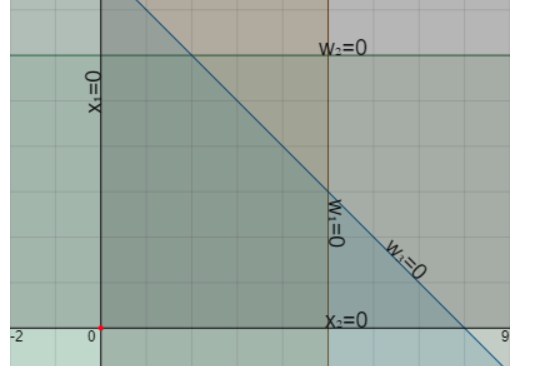
\includegraphics[scale=0.5]{mynd}
\end{center}
\paragraph{Skuggaverð} Ef ein skorða hækkar um eina einingu þá er hækkun hagn. Kallað skuggaverð. Heildar lausn - nýja heildarlausn / skorða - hækaðaskorða.
\paragraph{Nykurvending}
Ef það er gefin ný skorða fyrir dual verkefnið þá er bætt henni inn. Síðan er verkefnið set upp í fylki þar sem ekki tekið með slaka breytur í zmax. Síðan er fylkinu byllt og margfaltað með -1. Næst er framkvæmd vending fyrir nýju skorðun. Lausninn er fenginn með því að byllta fylkinu til baka og margfaladað með -1. 



\columnbreak
\textbf{Næmnigreining} \\
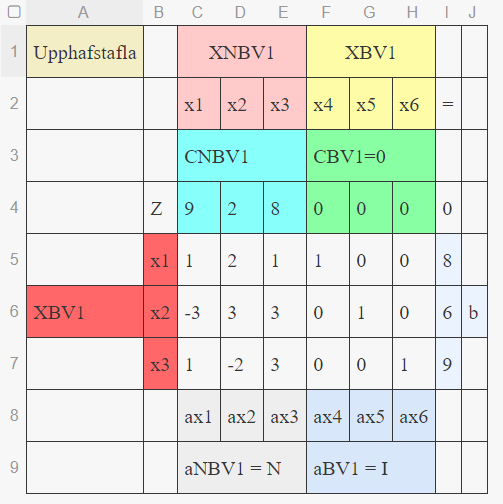
\includegraphics[scale=0.8]{upp}

\end{multicols}
\end{document}